\documentclass{bfh}
\usepackage[numbers]{natbib}
\usepackage[nohyperlinks]{acronym}

\title{Bachelor Thesis}
\subtitle{An Android Client for Bitmessage}
\author{Christian Basler}
\advisor{Kai Brünnler}
\expert{Daniel Voisard}
\date{\today}

\newcommand{\abbr}[1]{\textbf{#1}}

\begin{document}
  \lstset{language=Java}
  \maketitle

  \section*{Trademarks}
  Android and Google Play are trademarks of Google Inc.\\
  Oracle and Java are registered trademarks of Oracle and/or its affiliates.\\
  Other names may be trademarks of their respective owners.

  \section*{Abbreviations}
  \begin{acronym}[S/MIME ]
    \acro{CPU}    {central processing unit}
    \acro{GPU}    {graphics processing unit}
    \acro{POW}    {proof of work}
    \acro{OS}     {operating system}
    \acro{PGP}    {Pretty Good Privacy}
    \acro{MIME}   {multipurpose internet mail extensions}
    \acro{S/MIME} {Secure/\acs{MIME}}
    \acro{JDBC}   {Java database connectivity}
    \acro{SQL}    {structured query language}
    \acro{NoSQL}  {Not only \acs{SQL}}
    \acro{API}    {application programming interface}
    \acro{DOS}    {denial of service}
    \acro{nonce}  {number used once}
  \end{acronym}


  \newpage
  \section*{Abstract}
  If you don't want anyone snooping in your e-mails you might already encrypt your correspondence. But you still can't hide who you're writing to, and your e-mail client might even reveal much more about you, your computer, and the software you use. Bitmessage attempts to solve all this, but up until now there was no practical way to use it on mobile phones, which might be a downside when you're on the run.

  Bitmessage provides some unique challenges for mobile clients. Its users tend to be bordering on paranoia, or as often might really be tracked. The protocol is as wasteful as a hen; it needs both immense amounts of traffic and a lot of \acs{CPU} time. It works by distributing every message to every client, so they can pick up the ones they can decrypt with the available private keys. To protect the network from malicious flooding, a \acl{POW} is required, which is done by calculating a partial hash collision. So typically you'd want as many \acs{CPU} cores as possible, no shortage of electricity and a flat rate on internet access --- not quite the perfect basis for a mobile app.

  Apart from those protocol specific difficulties, Android\texttrademark{} has some challenges of its own. For example, to preserve memory and battery power, the \acl{OS} might kill practically any process at any time, especially those that just sit in the background and process incoming network objects. Then there are some major Java dependencies missing in the Android VM, most notably \acs{JDBC}, widely used for accessing databases. And finally, there are a lot of very different devices out there, some with processors hardly fast enough to browse the web and others as strong as some desktop computers.

  There were two main optimisations, both optional. Firstly, Android provides a highly optimized method to synchronize data with a server. Fortunately it was possible to leverage this while still using the official Bitmessage protocol. Secondly, for weaker phones an option to let a server do the \acl{POW} was added. For both options the user must give up some of his anonymity towards the server --- everything has its price.

  You can get more information about the app at \url{https://dissem.ch/abit}

  \begin{center}
    
\includegraphics[width=0.3 \textwidth]{images/QR_abit_webpage.pdf}
  \end{center}


  \newpage
  \tableofcontents


  \newpage
  \section{Introduction}

  \subsection{What is Metadata?}

  Metadata is information about data we create or access. This could be the websites we visit, what tv programmes we watch, or the sender, recipient, time, which mail client was used, maybe even where it was sent from and what anti-virus is used. The volume and quality of metadata greatly depends on the kind of data and the software used to create it.

  While encryption technology like \ac{PGP} or \acs{S/MIME} provides a secure way to protect content from prying eyes, it can't hide the header information: sender, recipient, subject and possibly much more.

  Ever since the revelations of whistleblower Edward Snowden we learned that metadata --- most notably information about who communicates with whom --- is equally interesting and much easier to analyse than the actual content.\cite{guardian:metadata}

  \subsection{How Can We Hide Metadata?}

  With e-mail, all metadata is plain text, even for encrypted messages. We might be able to encrypt the connection to the e-mail provider, and they might or might not encrypt their connections to other providers. We can only hope that both our and the recipient's e-mail provider are both trustworthy and competent. Can we really expect that from something we get for free? And can we be sure they're not forced to release what they know to some agency?\cite{yale:nsl}

  With Bitmessage we send a message to a sufficiently large number of participants, with the intended recipient among them. Content is encrypted such that only the person in possession of the private key can decrypt it. All participants try to do this in order to find their messages.

  \subsection{What is Bitmessage}
  
  Bitmessage is a peer to peer protocol building a mesh network among the participating clients. Every client tries to maintain multiple connections to other network nodes and has a full copy of every current object.
  
  Objects are encrypted using a public key. Every client tries to decrypt each object using its private keys, processing the ones where it succeeds.

  \subsubsection{Advantages}
  A big advantage of Bitmessage is its inherent key management. The address contains a hash of the public key, and retrieving said key is an integral part of the protocol.

  And the selling point of course is that everything is encrypted and signed, and there is next to no metadata an attacker could use.

  Finally, the setup is very easy. You just need to install a client software, there's no setup necessary except a click to create a new identity (i.e. Bitmessage address) if your client didn't do that when it started for the first time.

  \subsubsection{Disadvantages}
  Of course the protocol uses a lot of resources. The traffic problem could be somewhat managed by splitting it into streams\cite{wiki:stream}, but the \ac{POW} is required in order to protect the network.

  As you might guess, the protocol doesn't scale well. As the user base grows and traffic increases, it might be too much for weaker clients (read mobile phones) to process. Again, streams are said to be the solution, but if there's a big surge in network usage the implementations might not be ready. Unfortunately for this project, a successful mobile client might be responsible for that surge.

  If somehow your private key gets into wrong hands, they might be able to read every message you ever received, even if you deleted them locally. Nobody can prevent an entity from collecting all encrypted objects just in case the might be of value some day. They can't read the messages you've \textit{sent} though, unless they got your recipient's private key as well.

  On the usability side, the addresses aren't really human readable, and any method to make it look friendlier would either be complicated to set up or make the client insecure, or both. Then no client yet supports attachments, and there's still some controversy on how to implement them into the protocol. Large attachments wouldn't be possible anyway, due to message size restrictions and \ac{POW}.

  \subsubsection{Risks}
  As when you decide to use Tor, a software for enabling anonymous communication formerly known as 'The Onion Router', you might be flagged by some security agency as a possible threat.\cite{wired:tor} By itself this isn't necessarily a problem, but if you're a journalist it might be a risk for your informants, and combined with oder red flags you might be prevented from flying in or into the U.S.A.

  .

  .

  TODO


  \subsection{Motivation Behind this Thesis}
  \subsubsection{Current state -- what is missing?}
  Until recently there was no mobile client for Bitmessage, and the client that turned up since is very wasteful to the devices resources, draining the battery in little time. The alternative is to use an e-mail relay server, but this means to give up the private key to this server and end-to-end encryption is much more difficult to achieve. Therefore this might not be a viable option, especially if you can't run your own server.

  \subsubsection{How should it be?}
  We need mobile Bitmessage clients that allows the user to choose their levels of convenience, privacy and resource hunger. There will always be trade-offs between needed traffic, battery use and privacy, and for each user the answer might look slightly different.

  \subsubsection{Why is it hard to do?}
  Bitmessage is very wasteful with resources by design. All messages are being sent to and stored on all nodes, and to protect the network \ac{POW} is required for all objects that are distributed, meaning some very \acs{CPU}-heavy calculations need to be done. The protocol wasn't developed with mobile users in mind, and while smartphones are getting increasingly powerful, there is at least the issue of battery use to watch out for, and many users have limited traffic on their data plan.

  \subsubsection{Why me, and how do I intend to do it?}
  I have seven years of experience developing Java applications, and was programming Android apps from the moment I had my ``Android Dev Phone 1''. As I developed Jabit, a Java implementation of the Bitmessage client, as my last project, I also have great knowledge about the Bitmessage protocol.

  There are a few optimisations that I intend to do:
  \begin{itemize}
    \item Connect to only one reliable node instead of eight random nodes. This should reduce battery usage, but yields some risk if the node is compromised. Also, the node must forward all messages to all connected mobile clients instead of the default eight random nodes.
    \item Don't save objects we can't decrypt. We can solely save their hashes, but this means we're using the network without supporting it. This also might be an attack vector.
    \item Only connect to the network if we're on Wi-Fi and charging. This means of course that we'll only receive messages when we're connected with a Wi-Fi and charging.
  \end{itemize}
  Of course every option has its own drawbacks, so they will be configurable. As for the \ac{POW}: Jabit highly optimises its calculation, which might be enough for modern smartphones.

  Further optimisations might introduce a server component that \textit{might} do
  \begin{itemize}
    \item Proof of work
    \item Request public keys, requiring us to give up some anonymity towards the server.
    \item Inform the client about new messages sent to its addresses. This would mean to give up our anonymity towards the server in the best case (which isn't supported by the protocol yet), towards the whole network (which is somewhat supported), or give up the private key to the server (which, for many users, is unacceptable).
  \end{itemize}

  To find out what is actually necessary, a naive impementation will be done first.

  \subsection{The Jabit Bitmessage Library}
  Jabit has been developed as a preparing project for this thesis. It implements (most of) the Bitmessage protocol in Java and can therefore easily be used both for server applications as well as Android apps.

  Almost all alternative clients are based on PyBitmessage, which is somewhat inconvenient as it always requires PyBitmessage to run along with the client. This isn't really a problem on desktop computers, but might render creating  an easily deployable server application slightly more difficult, and is quite impractical on mobile devices.


  \subsubsection{Architecture}
  Jabit follows the Ports and Adapters architecture. There is a domain module which contains all the data types and most parts of the protocol implementation, and provides several ports, to which adapters can be attached. Adapters include the data repositories, \ac{POW}, network code and, more recently, cryptography (see \ref{subsec:bcvssc} \nameref{subsec:bcvssc}{}).

  \begin{center}
    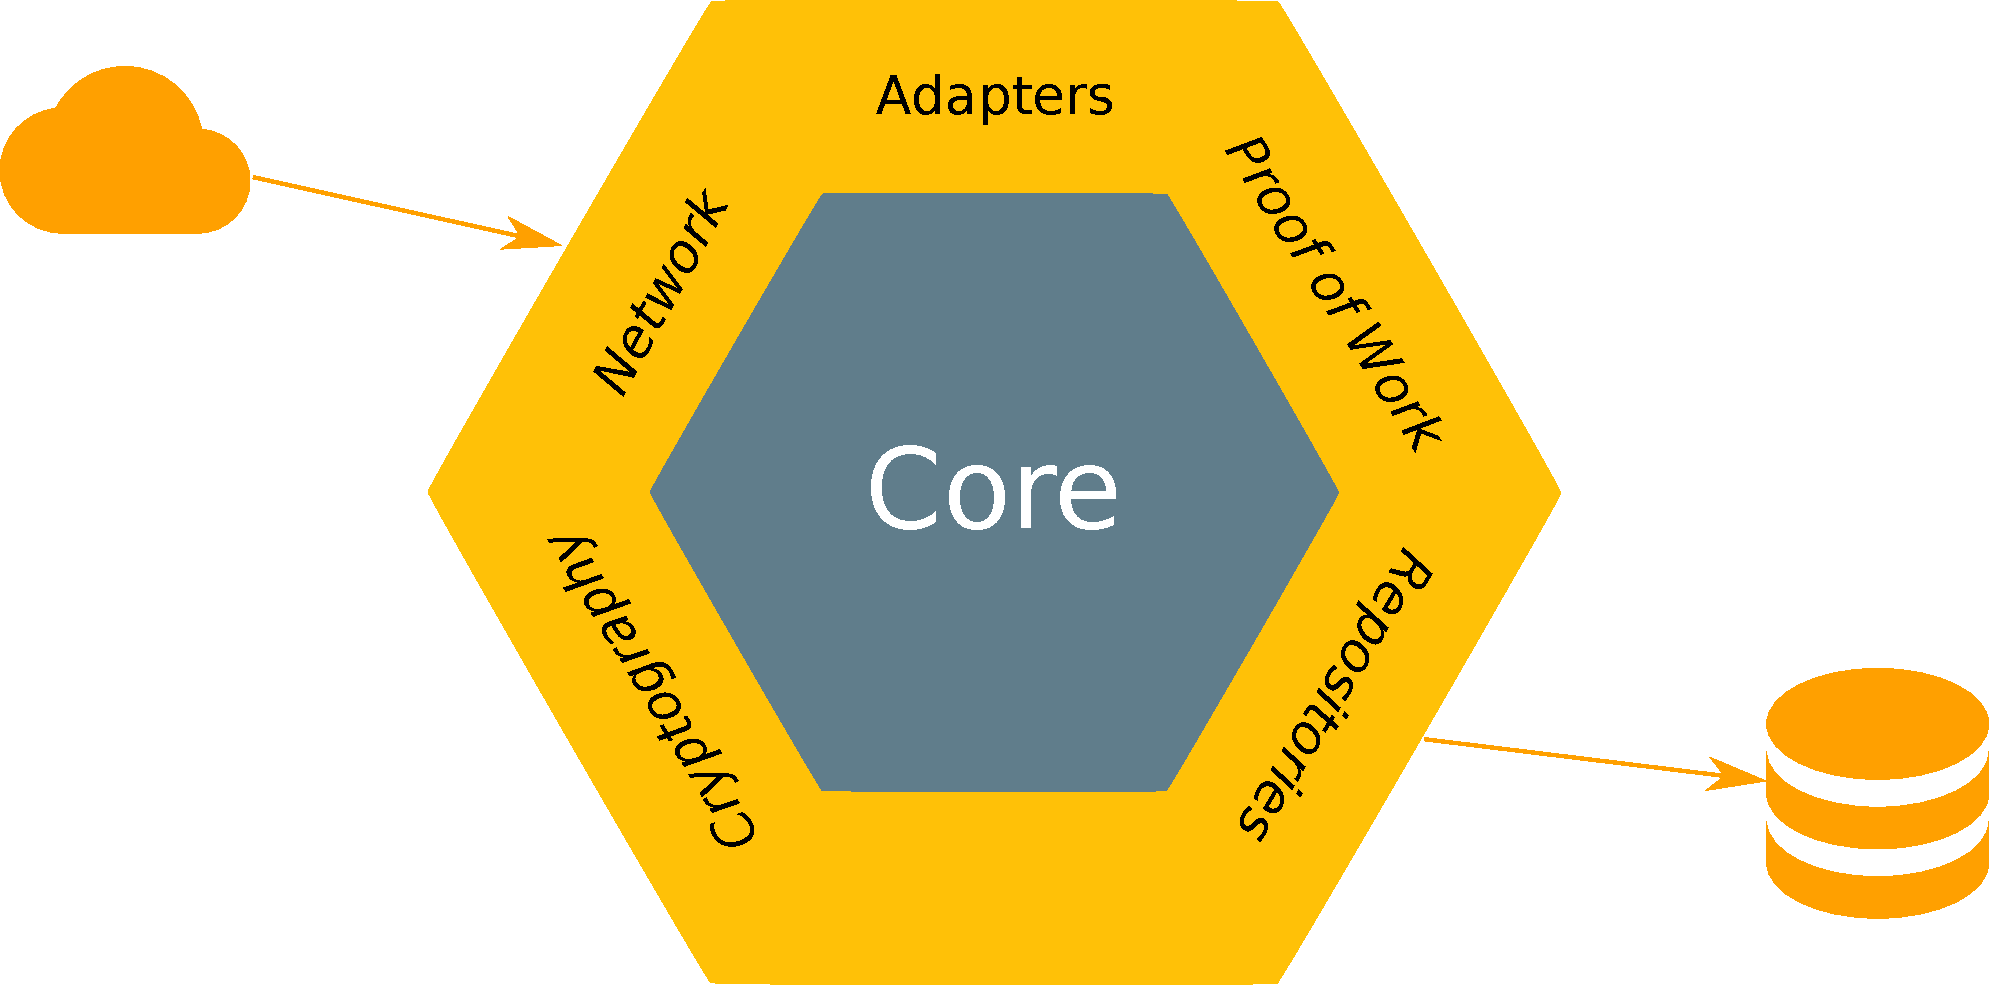
\includegraphics[width=0.5 \textwidth]{images/ports_and_adapters.pdf}
  \end{center}

  While there was hope to reuse the \acs{JDBC} implementation of the \textit{repositories}, it was clear that at some point someone might want to use a \acs{NoSQL} database or some other means of storage. Unfortunately, an Android specific implementation came first, as explained in section \ref{subsec:jdbc} \nameref{subsec:jdbc}.

  The \textit{\acl{POW}} adapter exists in a single- and a multithreading version. The first mainly exists to show the concept, while the second one currently is always used to do the calculation, albeit remotely on a server or wrapped in some Android compatibility code. A future immplementation that uses the \acs{GPU}, which sometimes have thousands of cores, might be magnitudes faster and could easily replace the current worker.

  The \textit{network} code was put in an adapter as some Android specific tweaks were expected. This turned out to be wrong, but it didn't slow down development and might facilitate a future rewrite of the network code, so it still seems to be a good desicion.

  The \textit{cryptography} adapter is a fine example why you should never rely on static helper classes. Rewriting the code to use an adapter was a pain and it wouldn't have been complicated to do it right the first time.


  \newpage
  \section{The Bitmessage Protocol}

  \subsection{Bitmessage Commands}

  Commands are messages between nodes, used to initialize a connection and exchange information about the network and available objects.

  
\includegraphics[width=\textwidth]{images/command.pdf}

  The \textbf{magic} is a number to mark the beginning of a command. It is set to \texttt{0xE9BEB4D9}, but \textit{could} be changed for test clients so they can't connect to the real network.

  A \textbf{command} defines how the payload looks like and what the node is supposed to do with it. The commands used by the Bitmessage protocol are \textit{version}, \textit{verack}, \textit{addr}, \textit{inv}, \textit{getdata} and \textit{object}. Their uses are specified in the Bitmessage Protocol Specification.\cite{wiki:protocol}

  \textbf{Size} defines how many bytes of payload need to be read.

  The \textbf{checksum} is used to discover transmission errors.

  \textbf{Payload} is the data that belongs to a command. It could be anything from empty to a complex object containing a message.


  \subsection{Bitmessage Objects}
  Objects are distributed throughout the network using the "object" command. With exception of some legacy objects, they are signed and encrypted.

  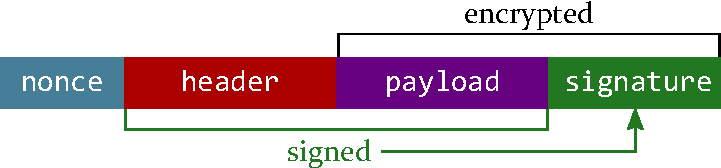
\includegraphics[width=\textwidth]{images/object.pdf}

  To prevent malicious flooding of the network and, to a lesser extent, spam, a \textbf{nonce} needs to be found such that a specific hash over the whole object represents a number lower than a calculated threshold. This is called \acf{POW}, and described in detail in section \ref{subsec:pow}.

  The object \textbf{header} consists of the expiration time, type and version of the object, and stream number. (Streams ar an optimisation feature of the protocol, so it should stay usable if many people start using Bitmessage.)
  
  The \textbf{payload} contains the actual data, depending on the message type.
  
  The \textbf{signature} covers everything except the nonce and is encrypted along with the payload, thus covering the unencrypted payload.

  There are four different types of objects in the Bitmessage protocol: \textit{getpubkey} is used to request a public key to some address, \textit{pubkey} contains said public key, \textit{msg} is a typical person-to-person message, and \textit{broadcast} is a message that is broadcast to anyone who subscribed to the sending address --- which needs to be known in order to subscribe.


  \subsection{Encryption}
  \label{subsec:encryption}
  Bitmessage uses elliptic curve cryptography for both signing and encryption. The math behind it is rather complicated, yet bases on the established principle to use a mathematical operation that has an inverse that is magnitudes more complicated than the operation itself. Instead of the typically used huge prime numbers, a point on an elliptic curve is multiplied by a high number.

  Advantages of elliptic curves is the fact that we don't need to search for big primes, but also that the keys can be much smaller while having the same encryption strength.

  The user, let's call her Alice, needs a key pair, consisting of a private key
$$k$$
which represents a huge random number, and a public key
$$K = G k$$
which represents a point on the agreed on curve -- by default that's \textit{secp256k1} for Bitmessage. Please note that this is not a simple multiplication, but the multiplication of a point along an elliptic curve. $G$ is the starting point for all operations on a specific curve.

  Another user, Bob, knows the public key. To encrypt a message, Bob creates a temporary key pair
$$r$$
and
$$R = G r$$
He then calculates
$$K r$$
uses the resulting Point to encrypt the message by calculating a double SHA-512 hash over the x-coordinate and sends $K$ along with the message.

  When Alice receives the message, she uses the fact that
$$K r = G k r = G r k = R k$$
so she just uses $R k$ to decrypt the message.

  The exact method used in Bitmessage is called Elliptic Curve Integrated Encryption Scheme or ECIES, which is described in detail on Wikipedia.\cite{wikipedia:ECC}\cite{wikipedia:ECIES}

  \subsection{Proof of Work}
  \label{subsec:pow}
  While invented as an anti spam feature, in Bitmessage \acf{POW} is mainly used to protect the network. Any malicious party could otherwise overload the network with an immense amount of messages, preventing other messages from being distributed and filling the hard disks of the weaker nodes, practically disabling the whole network. Therefore an object is only distributed to other nodes if its proof of work is correct and its time to live isn't up.

  The difficulty is calculated through a linear function of message size and time to live, i.e. a long lived message or a large one is more expensive to send, in terms of computation time.
$$ d = \frac{2^{64}}{n (l + \frac{t l}{2^{16}})} $$
\begin{tabular}{@{}>{$}l<{$}l@{}}
	d & target difficulty \\
	n & number of trials per byte \\
	l & payload length + extra byte \\
	t & time to live in seconds \\
\end{tabular}

  The virtual \textit{extra bytes} prevent flooding the network with a great number of extremely small objects by adding some minimal difficulty that's necessary to send a message.

  \textit{Time to live} can be up to 28 days, which is the default for \textit{pubkey} objects, but for normal messages two days are commonly used.

  To do the \acl{POW}, a \acs{nonce} must be found such that the first eight bytes of the object's hash (including \acs{nonce}) represent a smaller number than the target difficulty $d$.\\

\begin{lstlisting}
byte[] nonce = new byte[8]

do {
    nonce++
} while (
    lt(
      target,
      SHA512(SHA512(nonce + initialHash))
    )
);
\end{lstlisting}

  \listinginfo{}{initialHash}{a single SHA-512 hash over the whole object except for the nonce}{}
  \listinginfo{}{lt(a, b)}{a helper method that takes the first eight bytes of both arrays and returns \texttt{true} if the ones from $a$ represent a smaller number than the ones from $b$ and \texttt{false} otherwise}{}
  \listinginfo{}{+}{in this context, a concatenation of both arrays is meant}{[1, 2] + [3, 4] = [1, 2, 3, 4]}

  Note that this snipplet of pseudo code is optimised for readability. In a production implementation the loop should be as optimised (for speed) as possible, as it will be run so many times every nanosecond counts.


  \newpage
  \section{Naive Implementation}
  
  The naive implementation attempts to use the Jabit Bitmessage library as it is, with as little mobile optimisations as possible. The plan was to either discard or improve it afterwards. Fortunately, improvement was possible.

  \subsection{Unexpected Problems}
  Most problems can be summarised as this: Android builds on the Java language, but not on the Java platform. While the programming language is the same and most libraries can be used without any restrictions, there are some subtle differences that make a programmer's life hard --- some due to the limited resources of a mobile handset, others due to design decicions made by the Android development team.
  
  \subsubsection{Bouncy Castle vs. Spongy Castle}
  \label{subsec:bcvssc}
  Jabit heavily relies on Bouncy Castle, a very popular open source encryption library.\cite{bouncy} Sadly, Android ships with a broken version of Bouncy Castle. Even worse, when building an Android app, the toolchain just discards any Bouncy Castle dependencies in favour of the built-in, broken version.

  Some people recognised this problem, and built a fork of Bouncy Castle, called Spongy Castle. It basically just replaces “Bouncy” with “Spongy” wherever necessary, so it doesn’t get discarded during the build process. This works fine and is quite easily done. Unfortunately, it doesn’t work on the Desktop.

  The Oracle JVM requires Security Providers to be signed, which is done for Bouncy Castle builds, but not so for the Spongy derivation. As forking Jabit wasn’t an option, the whole cryptography part had to be refactored into an exchangeable module and implemented twice, in both a bouncy and a spongy manifestation.

  \subsubsection{JDBC}
  \label{subsec:jdbc}
  Android has its own API to access the included SQLite database. While it’s a nice, easy to use \ac{API}, the Android team didn’t deem it necessary to support \ac{JDBC}, which is the Java standard API to connect to databases.

  There is an open source project attempting to implement a \ac{JDBC} driver for Android’s SQLite database called SQLDroid, which looked very promising. But as it turned out, it lacks essential features, such as returning the automatically generated key of an inserted row. It doesn't even have the courtesy of throwing a NotImplementedException for missing features, instead it just doesn't do anything and returns \textit{null} where a result is required, making debugging unnecessarily tedious.\cite{github:sqldroid}

  Discovering SQLDroid was unfit for the job finally took more time than reimplementing all repositories using the Android database API. As they were already implemented as adapters, no change was necessary on the Jabit library. Many changes were made in the futile attempt to use JDBC though, most of them only to be reverted later on.

  \subsection{Expected Problems}
  Those problems were to be expected and need to be examined and possibly fixed as part of this thesis.

  \subsubsection{Proof of Work}
  Although modern smartphones tend to have faster processors than cheap personal computers, \ac{POW} for sending a public key takes more than 15 minutes on a device with four cores at 2.5 GHz. Even worse, during this time it uses so much power that the device discharges even when connected to a power supply.

  But as it used the default time to live of 28 days, cutting it down to two days shortened that time to a much more acceptable 1-2 minutes. Weaker devices still want to rely on a server to do their \ac{POW}, but for stronger devices and more paranoid people it might be a viable option.

  \subsubsection{Data Traffic}
  Not creating a full node that also distributes the objects it receives certainly reduces the necessary internet traffic, but a Bitmessage client still needs to download around 1 GiB of incoming objects each month.

  The relatively crude solution to this problem is an option to prevent connecting to the mobile network.

  \begin{center}
    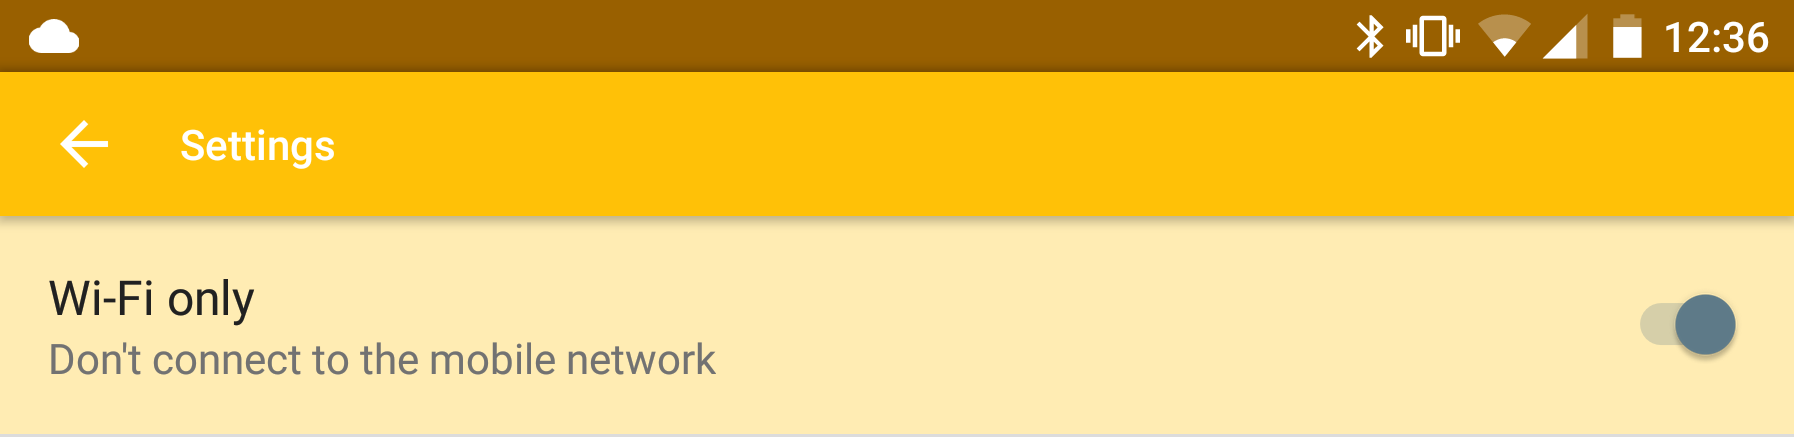
\includegraphics[width=0.8 \textwidth]{images/screenshot_wifi_only_setting.png}
  \end{center}

  \subsubsection{Storage}
  Limited storage isn't as big a problem as initially expected, experience showed that just barely over 100 MiB is used, wich isn't a problem on current smartphones.

  It shouldn't be too difficult to implement an option not to store any objects we don't need, but it certainly isn't a priority.


  \newpage
  \section{Android Specific Challenges}
  \subsection{Application Lifecycle}
  As with any good mobile system, Android doesn't hesitate to end any process of an application running in background, in order to save resources. Consequently anything that should be kept alive -- network connections and \ac{POW} come to mind -- needs special treatment. This is done through foreground services. The networking part and \ac{POW} hence needed to be moved into separate services. While not difficult, it needed some research to find out how it should best be done in our case.

  \begin{center}
    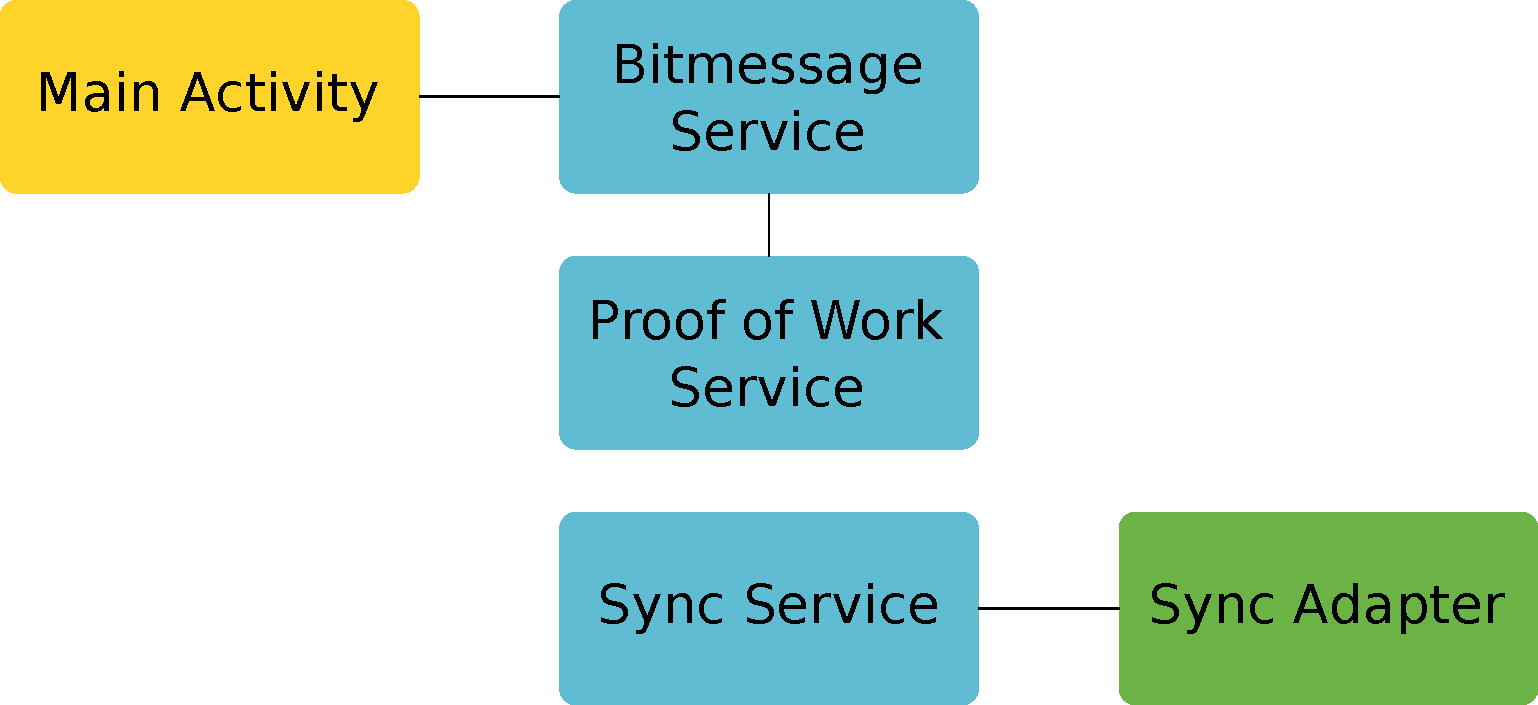
\includegraphics[width=0.8 \textwidth]{images/services.pdf}
  \end{center}

  It was decided to run all services as separate threads in the same process, which simplifies communication between those services, but has the risk of the whole app crashing if there is an error in a service.


  \newpage
  \section{Optimisations}
  \subsection{Sync Adapters}
  Android provides an API that can vastly reduce battery usage for apps that regularly update data over the internet. The system triggers synchronisation, so it can optimise its sleep modes. As it knows when the network access is done it can put the radio back to sleep immediately, unlike other kinds of network access where the system stays connected for some time in case a new connection needs to be established.

  Imagine five apps synchronising every five minutes, one after the other. In the worst case scenario the radio would need to wake up every minute, synchronize and could barely go back to sleep before the next app wants to synchronize.

  Although it's not intended, synchronisation can be done without any modifications to the Bitmessage protocol. What we need is a trusted node that is always available and therefore best run on a proper server. On successful connection all new messages are being exchanged, so we just need to connect, wait until new messages were exchanged, and then disconnect.

  As Jabit is a Java library, it was trivial to create a server application using Spring Boot and Jabit. It turned out though that it's necessary to limit the number of connections in a Bitmessage server, therefore connections are now being severed after 12 hours or when a limit of 100 connections is reached.

  \subsection{Server Side Proof of Work}
  To reduce power consumption and possibly reduce the time to send a message, \ac{POW} can be calculated by the synchronisation server. This feature needs some changes on both server and client, and some custom extensions to the protocol.

  \subsubsection{Initial Idea}
  The server accepts messages without \ac{POW}, which it will compute and fill in, and then relay that message. Of course this would leave the server extremely vulnerable to \ac{DOS} attacks -- an attacker could just send a bunch of messages and the server would be busy the rest of its life.

  Fortunately, Bitmessage has very secure authentication built in: every message is signed by a private key, and can be securely verified by anyone who knows the sender's address. We'll just send a message to the server that contains the actual message as content. All nonce fields are set to zero. Ther server checks if the sender is on a white list and then calculates the nonce and relays the complete message.

  A broadcast message would be best qualified for this task, as the client wouldn't have to be configured with a recipient address. The server is configured with a list of addresses that are allowed to request \ac{POW} and the client just needs to know the server's IP address or host name.

  \subsubsection{Acknowledging Issues}
  Unfortunately this approach has some issues. For one, sending a message would be very different using this method, requiring some major changes on the client side. Moreover, it would be impossible to generate acknowledgements.

  Acknowledgements are sent from the receiving client to notify the writer that the message was received. Think of it as a stamped addressed envelope delivered with a letter. The acknowledgement is part of the encrypted message the server can't read, so it couldn't calculate its \ac{POW}.

  Jabit doesn't support acknowledgements yet, but it would be a pity to prevent it by design.

  \subsubsection{\ac{POW} Protocol}
  Much of the planned design can be reused -- the encryption used by broadcasts, signing the messages -- but we need a wholly separate protocol, with some extra roundtrips to the server. Now the server just receives the parts needed for \ac{POW} calculation: a hash and a target value.

  When the nonce is found, it's saved on the database. The client will regularly poll for it (e.g. during synchronization cycles) until it retrieves the nonce.

  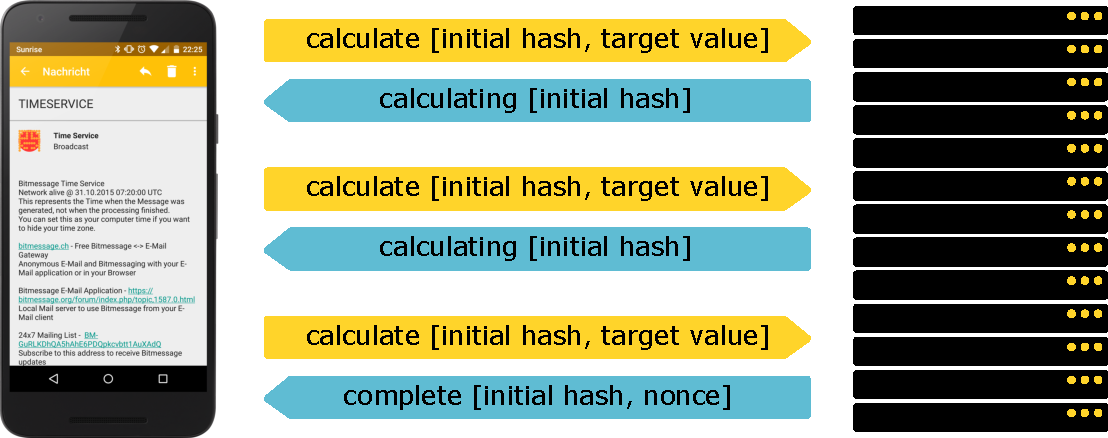
\includegraphics[width=\textwidth]{images/server_pow_protocol.pdf}

  For this feature, a new command was introduced, which needs to be implemented on both server and client. It has the same structure as any Bitmessage command, and \textit{custom} in the command field. As payload it contains a signed and encrypted block, containing the following structure:

  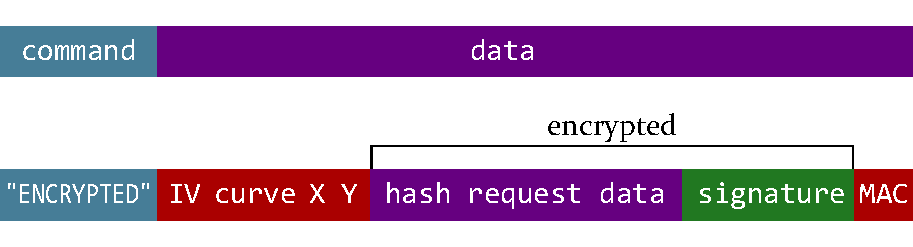
\includegraphics[width=\textwidth]{images/custom_message.pdf}

  The custom commands for the proof of work feature are encrypted and signed, including the kind of request or response. The \textit{command} field therefore always says \texttt{ENCRYPTED}. Afterwards comes the \textit{encryption header}, including the initialisation vector (IV), the curve type (should normally be 0x2CA), and the $X$ and $Y$ coordinates of a random public key (see \ref{subsec:encryption} \nameref{subsec:encryption}{}, variable $R$).

  The payload always consists of the initial hash (the base for \ac{POW} calculation) and the kind of request or response. The data field contains the target difficulty for the \texttt{CALCULATE} request, and the calculated nonce for the \texttt{COMPLETE} response. For the \texttt{CALCULATING} response data is an emtpy array.


  \newpage
  \section{The Finished App}












  \newpage
  \section{Comparison to Alternatives}
  \subsection{E-Mail Gateway}
  A free e-mail gateway can be found at \url{https://bitmessage.ch}.

  When using an e-mail gateway, you can use your preferred e-mail client, so we can assume that daily user experience is at least as good as with the native app. Setup isn't very complicated, but still not as easy as two taps for a new identity.

  As for security, we must really trust the gateway provider, because they possess our private key. Due to the way encryption is done in Bitmessage, there is no other way to solve this problem except for using \ac{PGP} or a similar product, but this is quite troublesome to set up and use for both parties.


  \subsection{Bitseal}
  Bitseal isn't available on Google Play\texttrademark{} anymore, but its sources can be found on Github:\\
  \url{https://github.com/JonathanCoe/bitseal}\\
  It isn't actively being developed right now, and unfortunately the servers needed for it to work aren't currently running. It would be possible to set up a private server, but this is out of scope of this thesis.

  As it aims to be a full Bitmessage client as well, Bitseal is more diractly comparable to Abit.

  \subsubsection{User Interface}
  \subsubsection{Settings}
  \subsubsection{Power Usage}








  \newpage
  \section{Social and Ethical Consequences}
  












  \newpage
  \bibliographystyle{plain}
  \bibliography{bibliography}

\end{document}